\chapter{無線LANセキュリティ演習}

\section{DoS攻撃}

\subsection{概要}

無線LANはその利便性のゆえに,現在広く一般に普及している.
しかし,無線による通信を行うことから,盗聴や侵入など,様々な攻撃に晒されてしまうという問題点がある.

この実習では,無線LANに対する代表的な攻撃の例としてDoS攻撃を取り上げ,実際に攻撃行ってその影響を観察した後,DoS攻撃への対策を考案した.

\subsection{実習内容}

\subsubsection{実習設備および実習環境}
使用したノートパソコンの一覧を表\ref{HW}に示す.

また,使用したソフトウェアは以下の通りである.

\begin{itemize}
  \item OmniPeek Personal(Windows用ソフトウェア)
  \item K-MAC(Windows用ソフトウェア)
  \item Aircrack-ng(BackTrack5用ソフトウェア)
\end{itemize}

\begin{table}[htsp]
  \caption{使用したノートパソコン一覧}
  \begin{tabular}{|c|c|} \hline
    機種名 & 備考 \\ \hline \hline
  \shortstack{\\ Mouse Computer S222X } & \shortstack{\\ 以下のOSがインストール済み \\ Kali Linux 1.0.7 Debian GNU/Linux(Kali Linux 1.0.7)\\ BackTrack 5 R3 Ubuntu 10.04.3 LTS \\ Ubuntu 14.04 LTS Ubuntu \\ Windows8} \\ \hline
  \shortstack{\\ Dell Inspiron 15R } & \shortstack{\\ 以下のOSがインストール済み \\ Kali Linux 1.0.3 \\ BackTrack 5 R3 \\ Ubuntu 13.04 \\ Windows8} \\ \hline
  \shortstack{\\ Mouse Computer s200} & \shortstack{\\ 予備機 \\ 以下のOSがインストール済み \\ Windows XP \\ BackTrack4} \\ \hline
  \end{tabular}
  \label{HW}
\end{table}

実験環境の概要図を図\ref{zikken}に示す.BackTrackを搭載したPC1台とWindowsを搭載したPC1台を攻撃用とし,それ以外のPC間でアクセスポイントを介してpingコマンドなどにより無線通信LAN通信を行う.

\begin{figure}
  \hspace*{\fill}
  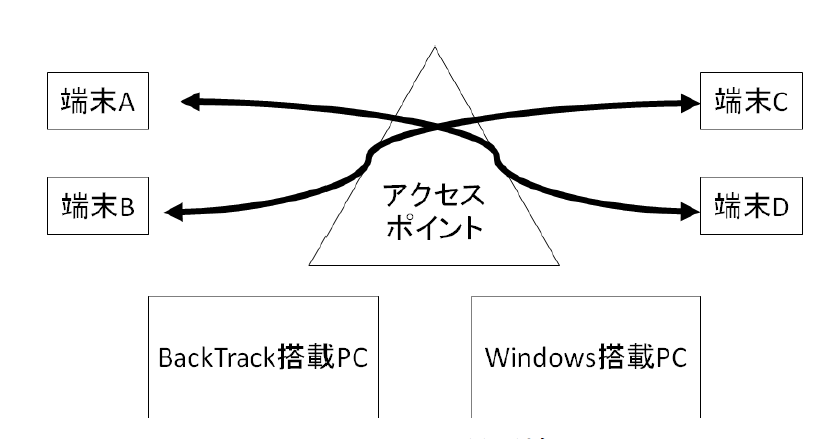
\includegraphics[scale=0.6]{MM01}
  \hspace*{\fill}
  \caption{実習環境}
  \label{zikken}
\end{figure}

\subsubsection{実習の手順}

\begin{itemize}
\item Windows搭載の攻撃用PCを用い,アクセスポイントを介し,正常な無線LAN通信を行っている端末間の通信を解析する.ソフトウェアはOmniPeekおよびK-MACを用いる.
\item 通信の解析により,攻撃者がフレームを送信するために必要となる情報,たとえば端末やアクセスポイントのMACアドレス,BSSIDなどを収集する.
\item 収集した情報を解析し,それを基にBackTrack搭載PCからaireplay-ngコマンドを用いてdisassociateフレームを送出し,端末間通信への影響を調べる.
\item 送信元,送信先のパターンを変更した場合の影響を調べる.
\item アクセスポイントのセキュリティ設定を変更した場合の影響を調べる.
\item disassociateフレームの代わりにdeauthenticationフレームを用いた場合について調べる.
\end{itemize}

\subsection{考察}
無線端末の接続状態は,大きく分けて3段階に分かれる.
認証も接続もなされていない状況,認証のみなされている状況,認証および接続がなされている状況の3つである.
正常な通信が行われている時,端末は認証および接続がなされている状況にある.

ここで,攻撃者がDoS攻撃を行ってdisassociateフレームを送出すると,受信した端末は接続終了が要求されたものとして接続を切り,認証はなされるが接続されていない状態へと遷移する.
このため,通常な通信が途中で一時的に切断されしまい,再度接続が行われるまで切断状態は継続することになる.

さらに,disassociateフレームでなくdeauthenticationフレームを創出した場合には,受信端末は認証も接続もなされていない状態へと遷移する.
このため,再度認証を行う処理と再度接続を行う処理の両方を行わなければならず,disassiciateフレームの送出によるDoS攻撃よりも影響は大きくなる.

無線端末の状態遷移を図\ref{tanmatu}に示す.

\begin{figure}
  \hspace*{\fill}
  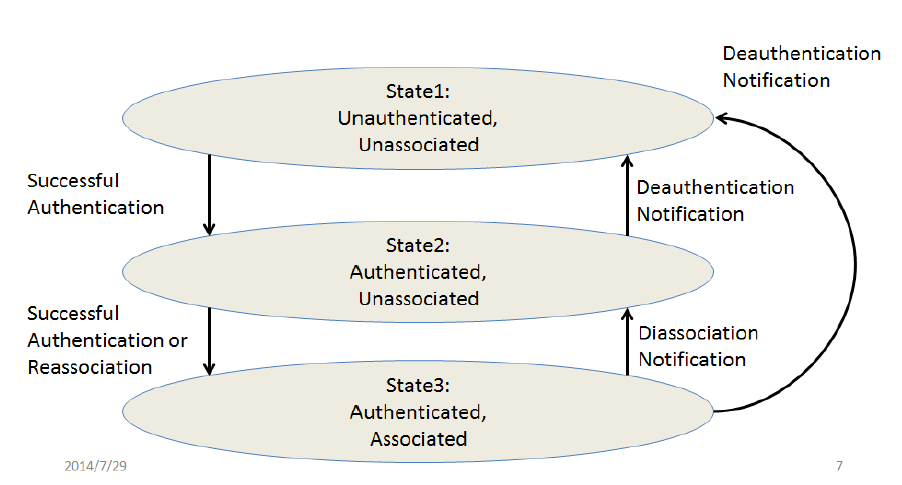
\includegraphics[scale=0.6]{MM02}
  \hspace*{\fill}
  \caption{無線端末の通信状態遷移図}
  \label{tanmatu}
\end{figure}

このように,収集した情報から,管理フレームを偽装して攻撃を行うことがDoS(Denial os Service)攻撃の近年の主流となっている.
今回,私の班では,多量のパケットを周辺ネットワークに投入することにより通信を阻害するというDoS攻撃の一手法を主に念頭に置いて実習を行ったため,管理フレームの偽装を行う手法についてはあまりデータを得ることはできなかった.

前述した,管理フレームを偽装する手法への対策としては,パケットが傍受されても内部情報を読み取られないように堅牢な暗号化手法を用いる,パケットの本来の送信者を確実に認識する何らかの手法を用いる,などが考えられる.

\section{WEPキーの解読}

\subsection{概要}

この実習では,Aircrack-ngを用いて無線LANのWEPキーを解読した.
また,解読したWEPキーを用いて盗聴したパケットを復号し,通信の内容を読み取れることを
確認した.

\subsection{実験内容}

\subsubsection{実験環境}

実験には,WEP暗号化に対応した無線LANルータと,無線LANクライアント機能を備えた2台のノートPCを用いた.

\begin{itemize}
\itemsep1pt\parskip0pt\parsep0pt
\item
  無線LANルータ:
  ルータモードで動作させ,13文字のパスワードによるWEP暗号化を設定した.インターネットや他のネットワークには接続せず,独立したネットワークを構築した.
\item
  ノートPC1:
  このPCは,WEPキーの解読に必要なパケットを発生させるために使用した.ノートPC1は,無線LANルータのIPアドレスへpingを送り続けるように設定した.
\item
  ノートPC2:
  このPCで,Aircrack-ngを実行し,実際にWEPキーの解読を行った.
\end{itemize}

\subsubsection{実験手順(WEPキーの解読)}

\begin{enumerate}
\def\labelenumi{\arabic{enumi}.}
\itemsep1pt\parskip0pt\parsep0pt
\item
  \texttt{airmon-ng}で使用できる無線LANインターフェースカードの一覧を表示した.
\item
  \texttt{airmong-ng}で無線LANインターフェースカードをモニタモードに投入した.
\item
  \texttt{airodump-ng}で通信できる無線LANアクセスポイントの一覧を表示し,解読対象の無線LANルータのBSSIDとチャネルを調べた.
\item
  \texttt{airodump-ng}を3.で調べたBSSIDとチャネルを指定して起動し,パケットのキャプチャした.
\item
  \texttt{airodump-ng}を実行した状態で,\texttt{aircrack-ng}を起動し,解読した.
\end{enumerate}

\subsubsection{実験手順(通信の盗聴)}

\begin{enumerate}
\def\labelenumi{\arabic{enumi}.}
\itemsep1pt\parskip0pt\parsep0pt
\item
  \texttt{airodump-ng}で対象の無線LANルータのパケットをキャプチャした.
\item
  実験手順(WEPキーの解読)の手順に従いWEPキーを解読した.
\item
  \texttt{airdecap-ng}にキャプチャファイルと解読したWEPキーを与え,キャプチャファイルを復号した.
\item
  復号したキャプチャファイルをWiresharkで開いた.
\end{enumerate}

\subsection{実験結果}

無線LANルータに設定した13文字のWEPキーは,\texttt{aircrack-ng}を起動してから約5分弱で正しく解読することができた.また,解読したWEPキーを用いてキャプチャしたパケットを解読したところ,HTTP通信などを解読することができた.

\subsection{考察}

WEP(Wired Equvivalent Privacy)はRC4(Rivest Cipher
4)を暗号化に用いている.RC4は同じ暗号鍵で異なる鍵ストリームを生成するために,IV
(Initialization Vector, 初期化ベクトル)
というものを用いている.この初期化ベクトルは24bitの長さしか持たないため,トラフィック量が多いと,同じ初期化ベクトルが再利用される可能性がある.また,平文のIPヘッダやSNAPヘッダが予測可能である事実も存在する.これらの脆弱性を活用し,統計的なアルゴリズムによりAircrack-ngはWEPキーを短時間で解読することが可能である.

\begin{figure}[htbp]
    \begin{center}
        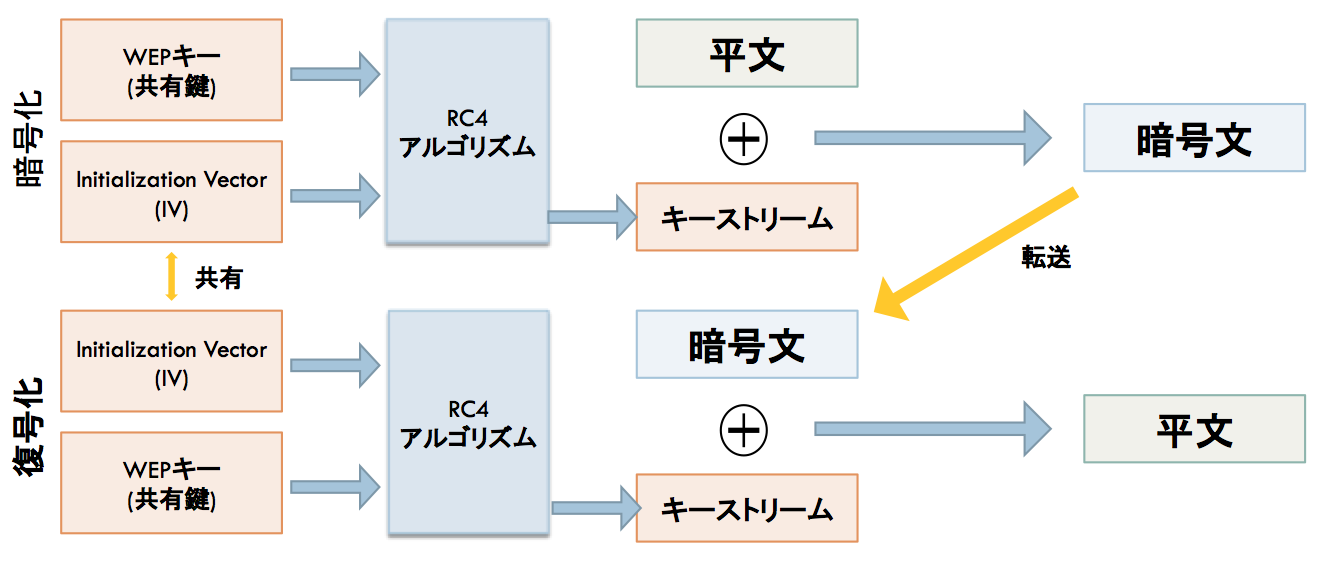
\includegraphics[width=120mm]{wep.png}
    \end{center}
    \caption{WEPの暗号化アルゴリズムの概要}
\end{figure}

今回の実験で確認したように,WEPキーは簡単に解読することが可能であり,セキュリティ上のリスクとなり得る.これを防ぐために,暗号化方式をWEPから,802.11iで定義されているWPA2-PSK
(AES)やWPA2-EAP(AES)
に置き換えることが効果的である.ただし,WPA2も辞書攻撃に対する脆弱性が存在するために,予測不可能で十分に長いパスフレーズを選択することが重要である.しかし,デバイスがレガシーであるなど,諸々の事情によりやむを得ずにWEPを使用しなければいけない状況もある.そのような場合には,TLS
(Transport Layer Security),VPN(Virtual Private Network)
,SSHトンネリングなど,上位層における暗号化によりある程度安全性を確保することが可能である.
